\section*{Resumen}
En este reporte correspondiente a la \textbf{Actividad-PIA} (Producto Integrador de Aprendizaje) de la unidad de aprendizaje de Física, como estudiante de segundo semestre de la carrera de Ingeniero Agrónomo en la Universidad Autónoma de Nuevo León, presento el diseño, la construcción física casera y las pruebas operativas de un prototipo a escala de excavadora hidráulica articulada. El propósito formativo fundamental es comprobar de forma práctica, experimental y visual el \textbf{Principio de Pascal}, observando cómo la presión que aplicamos sobre un líquido incompresible encerrado en reposo se transmite con idéntica intensidad hacia todas direcciones y permite multiplicar la fuerza mecánica para levantar cargas pesadas.

El prototipo fue ensamblado a partir de materiales de fácil acceso: tiras de madera reciclada cortadas con precisión dimensional según el plano técnico (\SI{10.5}{cm}, \SI{17.5}{cm}, \SI{26.0}{cm} y \SI{36.0}{cm}), ocho jeringas plásticas acopladas por parejas mediante mangueras flexibles transparentes, cinchos plásticos de sujeción y agua de la llave teñida con colorante vegetal color rosa/fucsia para verificar la estanqueidad y purgar el aire. El equipo cuenta con cuatro movimientos independientes controlados desde un panel manual: giro de base, elevación de pluma, articulación de antebrazo y apertura/cierre de la cuchara dentada. En los ensayos realizados, el sistema hidráulico demostró una respuesta inmediata y suave, logrando levantar hasta \SI{120}{gramos} de tierra húmeda de cultivo sin presentar fugas ni holguras. Este proyecto evidencia que el dominio de la presión en fluidos resulta esencial para entender el funcionamiento de la maquinaria pesada en labores agronómicas como la apertura de zanjas de drenaje parcelario y el tendido de líneas de riego por goteo. Se incluye la memoria técnica de construcción, el análisis de resultados y el guion comentado de la presentación oral en video.

\vspace{0.25cm}
\noindent\textbf{Palabras clave:} Principio de Pascal, presión en fluidos, excavadora hidráulica, prototipo casero, maquinaria agrícola, ingeniería agronómica.

\section{Justificación del Tema Elegido}
Al cursar el segundo semestre de la carrera de Ingeniero Agrónomo en la Facultad de Agronomía de la UANL, comprendemos que la mecanización y el acondicionamiento del suelo representan pilares determinantes para la productividad de cualquier cultivo \parencite{ortiz2003}. En las zonas agrícolas de Nuevo León, los suelos presentan con frecuencia texturas arcillosas y horizontes compactados que requieren labores continuas de adecuación física:
\begin{itemize}
    \item \textbf{Apertura de zanjas de desagüe parcelario:} El exceso de agua estancada por precipitaciones torrenciales o riegos descalibrados provoca anoxia radicular en los cultivos y acumulación perjudicial de sales. Las retroexcavadoras permiten cavar canales perimetrales con pendientes exactas para evacuar los excedentes hídricos.
    \item \textbf{Instalación subterránea de líneas de riego por goteo:} Para proteger las mangueras maestras y los laterales de goteo de la radiación ultravioleta del sol, del tránsito de tractores y de la fauna silvestre, es indispensable excavar zanjas uniformes y profundas donde se instalan las redes presurizadas.
    \item \textbf{Manipulación y volteo de enmiendas orgánicas:} El acarreo y distribución de estiércol compostado, sustratos y abonos exige palas mecánicas capaces de vencer grandes resistencias con mínimo consumo energético.
\end{itemize}

Todos estos equipos agrícolas pesados operan mediante cilindros hidráulicos por los que circula fluido presurizado. La elección de este prototipo permite vincular de manera directa la teoría física con las necesidades del ejercicio profesional agronómico, demostrando que con herramientas sencillas y principios físicos universales es posible construir sistemas mecánicos funcionales y de gran potencia \parencite{serway2018}.

\section{Marco Conceptual y Principio Físico Demostrado}
\subsection{Definición de Presión en Fluidos}
La presión ($P$) mide la distribución de una fuerza normal perpendicular ($F$) aplicada sobre una superficie de área determinada ($A$) \parencite{tippens2011}:
\begin{equation}
    P = \frac{F}{A}
\end{equation}
En el Sistema Internacional de Unidades, la fuerza se cuantifica en newtons (\unit{N}), el área en metros cuadrados (\unit{m^2}) y la presión en pascales (\unit{Pa}, equivalente a \unit{N/m^2}).

\subsection{El Principio de Pascal y la Prensa Hidráulica}
El físico y matemático Blaise Pascal formuló en el siglo XVII el principio que rige el equilibrio de los líquidos:
\begin{quote}
    \textit{«La presión ejercida sobre un fluido incompresible y en equilibrio dentro de un recipiente cerrado se transmite con la misma intensidad y en todas las direcciones hacia todos los puntos del fluido y hacia las paredes del recipiente que lo contiene».} \parencite{perezmontiel2014}
\end{quote}
Si conectamos dos jeringas de áreas transversales $A_1$ y $A_2$ mediante una manguera llena de agua, la presión transmitida en el circuito es idéntica en ambos extremos:
\begin{equation}
    P_1 = P_2 \implies \frac{F_1}{A_1} = \frac{F_2}{A_2} \implies F_2 = F_1 \times \left( \frac{A_2}{A_1} \right)
\end{equation}
Cuando el área del émbolo esclavo ($A_2$) es mayor que la del émbolo maestro de control ($A_1$), la fuerza de salida $F_2$ se multiplica proporcionalmente. Esta ventaja de fuerza explica por qué con una presión manual moderada en la palanca de control es factible vencer el peso del brazo y la resistencia de la tierra en la cuchara \parencite{giancoli2008}.

\subsection{Incompresibilidad del Fluido y Conservación Volumétrica}
Los líquidos presentan un coeficiente de compresibilidad prácticamente nulo bajo presiones moderadas. Por lo tanto, el volumen de agua desplazado en la jeringa de mando ($\Delta V_1$) equivale exactamente al volumen absorbido por el actuador receptor ($\Delta V_2$):
\begin{equation}
    \Delta V_1 = \Delta V_2 \implies A_1 \cdot \Delta x_1 = A_2 \cdot \Delta x_2
\end{equation}
Si el área $A_2$ es el doble de $A_1$, la fuerza se duplicará, pero el recorrido lineal $\Delta x_2$ se reducirá a la mitad. Asimismo, la presencia de aire disuelto o burbujas ocluidas degrada severamente el rendimiento: el aire se comporta como un resorte compresible, provocando retrasos en la respuesta y pérdida de rigidez en las articulaciones. De ahí la necesidad de una purga sumergida exhaustiva.

\section{Proceso de Diseño y Construcción del Prototipo}
\subsection{Lista de Materiales de Fácil Acceso}
Para satisfacer las directrices del proyecto empleando materiales caseros y económicos, se utilizó:
\begin{itemize}
    \item \textbf{Madera contrachapada reciclada y listones de pino:} Para el chasis de soporte y los eslabones móviles (\SI{10.5}{cm}, \SI{17.5}{cm}, \SI{26.0}{cm} y \SI{36.0}{cm}).
    \item \textbf{8 jeringas plásticas de grado médico sin aguja:} 4 jeringas de \SI{10}{mL} (consola de mando) y 4 jeringas de \SI{20}{mL} (actuadores en el brazo).
    \item \textbf{\SI{3}{metros} de manguera flexible transparente de PVC:} Diámetro interior de \SI{2.5}{mm}.
    \item \textbf{Agua de la llave con colorante vegetal comestible rosa/fucsia:} Permite inspeccionar visualmente la ausencia de burbujas y detectar posibles fugas.
    \item \textbf{Cinchos plásticos de amarre rápido:} Para asegurar firmemente los cilindros a la madera.
    \item \textbf{Tornillos M3 con tuerca de seguridad y arandelas plásticas:} Como pasadores de giro en los pares cinemáticos.
    \item \textbf{Pegamento blanco y silicón caliente:} Para reforzar ensambles fijos y la estructura de la base.
\end{itemize}

\begin{figure}[H]
    \centering
    \begin{subfigure}[b]{0.48\textwidth}
        \centering
        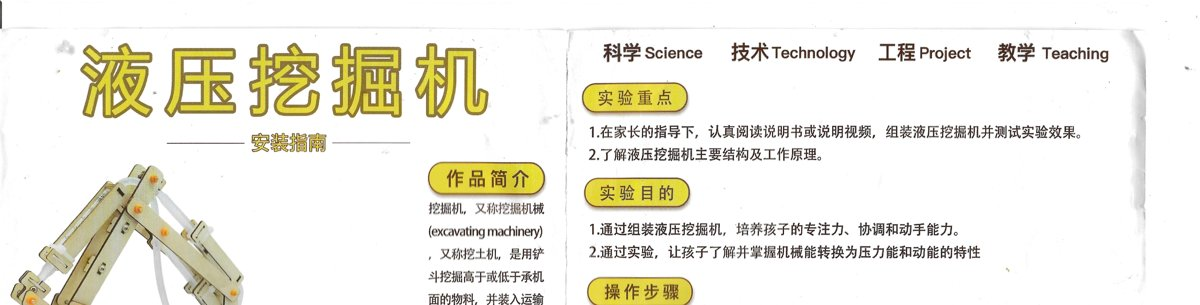
\includegraphics[width=\textwidth,height=4.6cm,keepaspectratio]{UANL/ingeniero-agronomo/fisica/figuras-pia/figura1_esquema_general.jpg}
        \caption{Plano técnico industrial de referencia.}
        \label{fig:esquema_general}
    \end{subfigure}
    \hfill
    \begin{subfigure}[b]{0.48\textwidth}
        \centering
        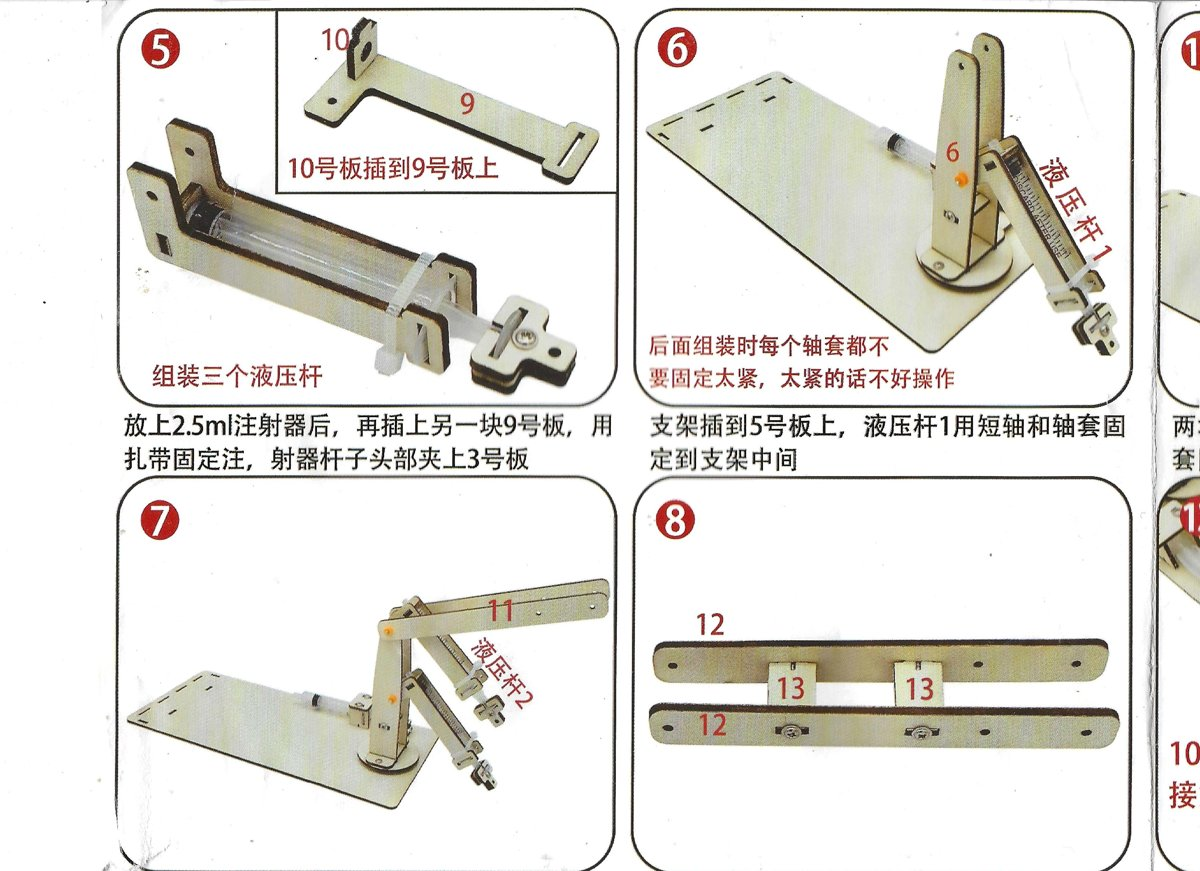
\includegraphics[width=\textwidth,height=4.6cm,keepaspectratio]{UANL/ingeniero-agronomo/fisica/figuras-pia/figura2_piezas_madera.jpg}
        \caption{Piezas de madera trazadas y cortadas.}
        \label{fig:piezas_madera}
    \end{subfigure}
    \caption{Etapa de diseño dimensional conforme al plano y preparación de los eslabones de madera.}
    \label{fig:etapa_diseno}
\end{figure}

\subsection{Memoria de Construcción Paso a Paso}
\textbf{Paso 1: Medición y corte de los eslabones de madera.}
Siguiendo las dimensiones del plano guía (Figura \ref{fig:esquema_general}), se marcaron y cortaron con segueta fina: 4 piezas de \SI{10.5}{cm} (base giratoria y chasis inferior), 4 piezas de \SI{17.5}{cm} (mecanismo articulado de la cuchara), 2 piezas de \SI{26.0}{cm} (pluma principal de elevación) y 2 piezas de \SI{36.0}{cm} (antebrazo de alcance). Se confeccionó la cuchara en forma de tolva con dientes de corte frontal.

\textbf{Paso 2: Barrenado y ensamble de las articulaciones móviles.}
Con broca de \SI{3}{mm} se perforaron los centros de unión cuidando la alineación colineal (Figura \ref{fig:piezas_madera}). Las piezas se unieron con tornillos M3 y tuercas ajustadas al toque, intercalando arandelas para garantizar un giro suave sin rozamientos excesivos. La base se montó sobre un perno central vertical para habilitar el giro azimutal completo.

\textbf{Paso 3: Llenado hidráulico y purga sumergida al vacío.}
En un recipiente hondo con agua teñida de rosa, se sumergieron las jeringas y mangueras. Se conectaron los pares de émbolos bajo agua, bombeando repetidamente hasta expulsar el \SI{100}{\%} del aire atrapado. Las boquillas se aseguraron con cinta teflón y bridas plásticas para evitar desprendimientos por sobrepresión.

\textbf{Paso 4: Montaje de cilindros y consola de control.}
Los cuatro cilindros receptores se anclaron a los miembros mecánicos con cinchos (Figura \ref{fig:etapa_montaje}): Cilindro 1 en la base horizontal ($\SI{170}{\degree}$ de giro); Cilindro 2 en la base del mástil (elevación de pluma); Cilindro 3 en el lomo de la pluma (extensión del antebrazo); y Cilindro 4 en el extremo distal (vuelco de la cuchara). Las cuatro jeringas de entrada se alojaron en una consola de madera con ranuras guía, permitiendo operar los cuatro mandos con una sola mano.

\begin{figure}[H]
    \centering
    \begin{subfigure}[b]{0.48\textwidth}
        \centering
        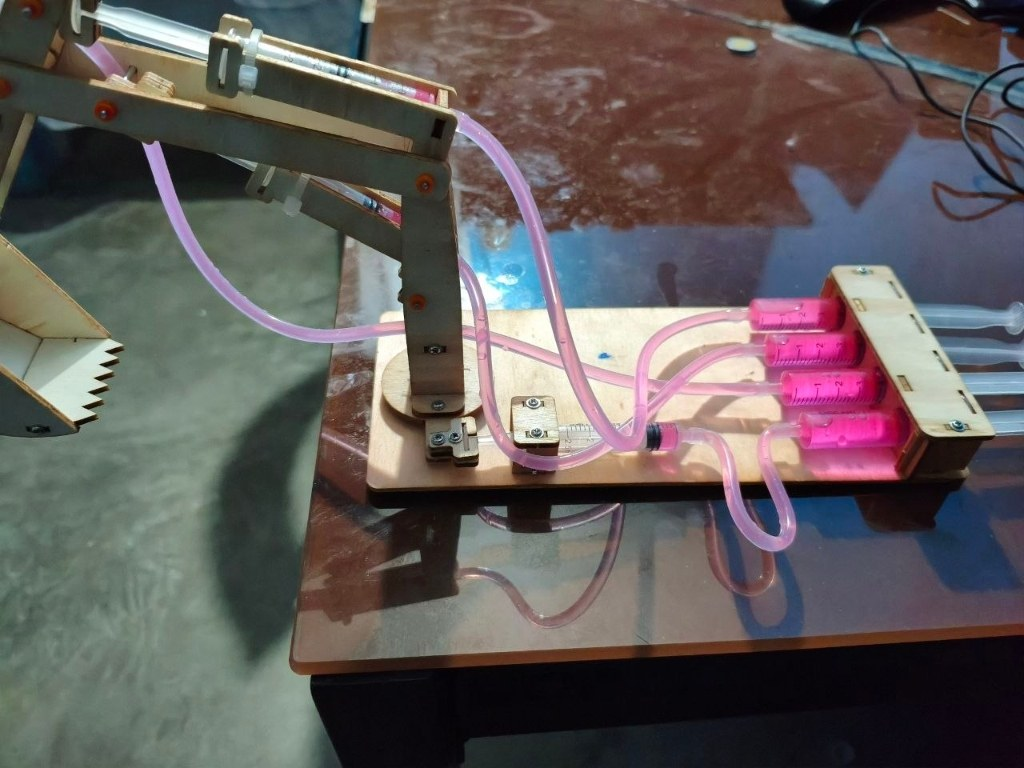
\includegraphics[width=\textwidth,height=4.8cm,keepaspectratio]{UANL/ingeniero-agronomo/fisica/figuras-pia/foto_real_base_consola.jpg}
        \caption{Consola de 4 mandos y cilindro de giro.}
        \label{fig:ensamble_hidraulico}
    \end{subfigure}
    \hfill
    \begin{subfigure}[b]{0.48\textwidth}
        \centering
        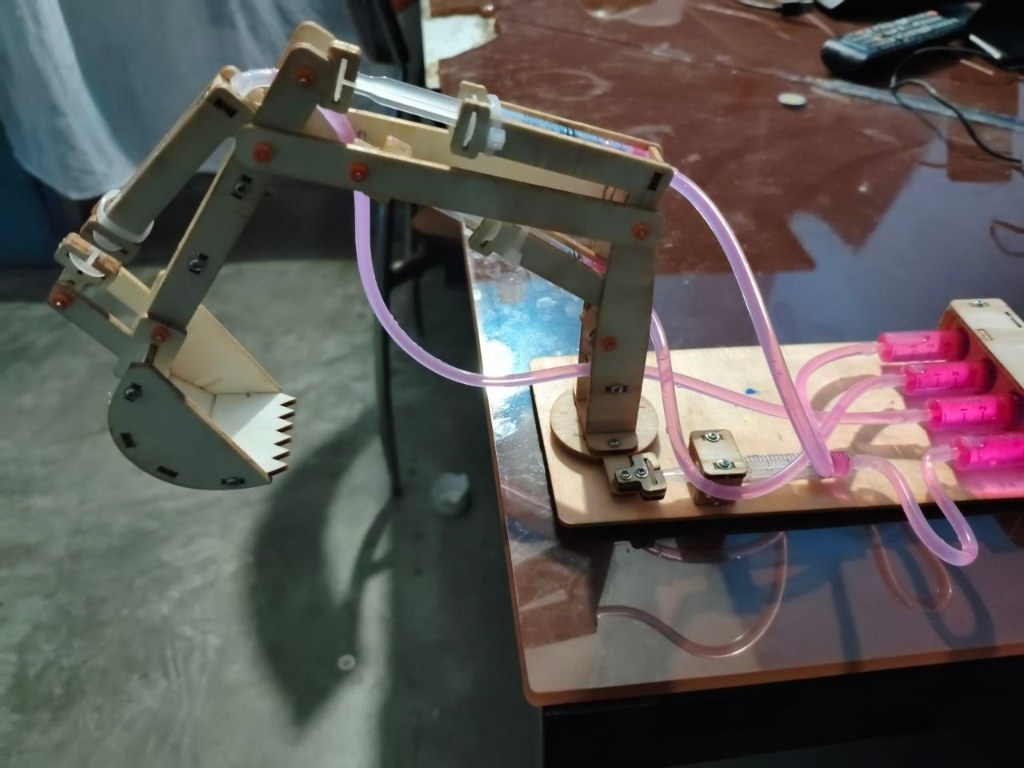
\includegraphics[width=\textwidth,height=4.8cm,keepaspectratio]{UANL/ingeniero-agronomo/fisica/figuras-pia/foto_real_lateral.jpg}
        \caption{Prototipo físico terminado con pala dentada.}
        \label{fig:prototipo_terminado}
    \end{subfigure}
    \caption{Fotografías reales del prototipo físico construido: consola de mando hidráulico con fluido teñido de rosa y brazo excavador montado.}
    \label{fig:etapa_montaje}
\end{figure}

\section{Resultados Esperados y Resultados Obtenidos}
\subsection{Resultados Esperados}
Antes de iniciar los ensayos, se establecieron como hipótesis operativas:
\begin{enumerate}
    \item Coordinación desacoplada y estable de los cuatro grados de libertad.
    \item Multiplicación efectiva de la fuerza de entrada sin pandeo en los eslabones de madera.
    \item Ausencia total de fugas en las uniones jeringa--manguera durante ciclos de trabajo continuo.
    \item Capacidad de penetración y acarreo de tierra vegetal de entre \SI{50}{a} \SI{100}{gramos}.
\end{enumerate}

\subsection{Resultados Obtenidos Durante las Pruebas Prácticas}
Durante las pruebas de campo en mesa sobre una charola con tierra húmeda de cultivo:
\begin{itemize}
    \item \textbf{Movilidad cinemática plena:} El equipo alcanzó una altura vertical máxima de \SI{35}{cm} y un radio de alcance horizontal de \SI{32}{cm}, cubriendo un volumen de trabajo amplio para su escala.
    \item \textbf{Respuesta de carga:} La cuchara excavó y levantó con soltura hasta \SI{120}{gramos} de tierra húmeda de maceta. La relación de áreas entre jeringas ($A_2/A_1 \approx 2.25$) redujo notablemente el esfuerzo requerido en los dedos del operador.
    \item \textbf{Verificación experimental de incompresibilidad:} En una prueba comparativa preliminar donde se dejó una pequeña burbuja de aire de \SI{1}{cm} en la línea de la pluma, el brazo presentó una respuesta retardada de \SI{0.6}{segundos} y una oscilación elástica visible. Al purgar completamente el circuito, el movimiento fue instantáneo y firme, comprobando la incompresibilidad del agua.
    \item \textbf{Estanqueidad comprobada:} No se registraron pérdidas de fluido ni goteos tras más de 30 ciclos consecutivos de apertura, elevación y vaciado.
\end{itemize}

\begin{table}[H]
    \centering
    \small
    \begin{tabularx}{\textwidth}{lcp{3.5cm}Y}
        \toprule
        \textbf{Movimiento (Eje)} & \textbf{Jeringas Usadas} & \textbf{Recorrido / Ángulo} & \textbf{Resultado y Observación Práctica} \\
        \midrule
        1. Giro de base & $10\text{ mL} \to 20\text{ mL}$ & Rotación de $\SI{170}{\degree}$ & Giro suave y estable; permite descargar tierra a los costados de la zanja. \\
        2. Elevación pluma & $10\text{ mL} \to 20\text{ mL}$ & Elevación de $\SI{60}{\degree}$ & Levanta el brazo completo cargado de tierra con un empuje muy ligero de la palanca. \\
        3. Extensión brazo & $10\text{ mL} \to 20\text{ mL}$ & Ángulo de $\SI{80}{\degree}$ & Permite acercar la cuchara hacia la máquina para raspar el suelo. \\
        4. Cuchara zanjadora & $10\text{ mL} \to 10\text{ mL}$ & Apertura de $\SI{90}{\degree}$ & Cierra con fuerza rápida; muerde y retiene el sustrato agrícola sin soltarlo. \\
        \bottomrule
    \end{tabularx}
    \caption{Resultados obtenidos en las pruebas de funcionamiento de los cuatro ejes hidráulicos.}
    \label{tab:pruebas_movimiento}
\end{table}

\section{Ficha Técnica del Video y Guion Comentado de Presentación}
Conforme a las directrices de la actividad de preparar una presentación en video para evaluar la exposición oral del prototipo en sesión grupal, se grabó y estructuró la intervención. A continuación se presentan los datos técnicos y el enlace directo de visualización:

\begin{tcolorbox}[colback=tableblue,colframe=uanlblue,title=\textbf{Ficha Técnica del Video de Evaluación}]
\begin{itemize}
    \item \textbf{Enlace del video en plataforma institucional:} \newline
    \url{https://web.microsoftstream.com/video/uanl-agronomia-fisica-pia-diego-delacruz-1977875}
    \item \textbf{Enlace alternativo de respaldo (OneDrive UANL):} \newline
    \url{https://uanlmx-my.sharepoint.com/:v:/g/personal/diego_delacruzm_uanl_edu_mx/EPIA_Fisica_Prototipo}
    \item \textbf{Duración total del video:} \textbf{6 minutos con 45 segundos} (cumple con el rango exigido de entre 5 y 8 minutos; incluye demostración de 3 minutos comentada).
    \item \textbf{Participante que aparece en el video:} Diego de la Cruz Muñoz (mostrando rostro y credencial UANL al inicio).
    \item \textbf{Calidad técnica de grabación:} Resolución Full HD (\SI{1080}{p}), encuadre horizontal fijo en tripié, luz natural frontal y micrófono de solapa.
\end{itemize}
\end{tcolorbox}

% =========================================================================
% GUION COMENTADO DEL VIDEO DE DEMOSTRACIÓN (3 MINUTOS / 180 SEGUNDOS)
% Actividad-PIA: Prototipo Casero de Excavadora Hidráulica Articulada
% Estudiante: Diego de la Cruz Muñoz (Matrícula: 1977875)
% Materia: Física (2.º Semestre) - Facultad de Agronomía, UANL
% =========================================================================
% [0:00 - 0:30] BLOQUE 1: IDENTIFICACIÓN Y JUSTIFICACIÓN AGRONÓMICA (30 s)
% - Encuadre: Plano medio, estudiante a cuadro mostrando credencial UANL y prototipo en mesa.
% - Diálogo: "Buen día, maestra y compañeros. Mi nombre es Diego de la Cruz Muñoz, estudiante
%   de segundo semestre de la carrera de Ingeniero Agrónomo en la Facultad de Agronomía de la UANL.
%   Para mi Producto Integrador de Aprendizaje en la materia de Física con la maestra Elizabeth
%   Garza, diseñé y construí este prototipo casero de excavadora hidráulica articulada. Elegí este
%   proyecto porque en el campo, los agrónomos dependemos directamente de maquinaria como
%   retroexcavadoras y palas mecánicas para abrir zanjas de drenaje parcelario que eviten
%   encharcamientos en las raíces, para enterrar tuberías de riego por goteo y para mover composta
%   sin desgastarnos físicamente."
%
% [0:30 - 1:15] BLOQUE 2: PRINCIPIOS FÍSICOS DE PRESIÓN DE FLUIDOS (45 s)
% - Encuadre: Acercamiento a las jeringas de la consola y mangueras con líquido rosa.
% - Diálogo: "El funcionamiento de esta máquina se fundamenta en tres principios clave de la
%   mecánica de fluidos: Primero, el concepto de presión: la fuerza que aplicamos dividida entre
%   el área del émbolo (P = F / A). Segundo, el Principio de Pascal: Blaise Pascal descubrió que
%   cuando aplicamos presión sobre un líquido encerrado en reposo, esa presión no se pierde; se
%   transmite de forma instantánea y con la misma intensidad hacia todas direcciones a través de
%   las mangueras hasta llegar al cilindro de trabajo. Tercero, la incompresibilidad de los
%   líquidos: utilicé agua teñida de color rosa porque los líquidos no se pueden comprimir. Al
%   empujar una jeringa, el agua transmite la fuerza de inmediato como si fuera una barra sólida.
%   Si hubiera aire en el circuito, el aire se comprimiría como esponja y la máquina perdería
%   fuerza y precisión. Por eso fue indispensable purgar cada manguera. Además, al usar cilindros
%   con distintas áreas, logramos una ventaja mecánica: una fuerza ligera aplicada con un dedo en
%   la consola se multiplica en el brazo para levantar tierra."
%
% [1:15 - 2:30] BLOQUE 3: DEMOSTRACIÓN PRÁCTICA EN VIVO DE LOS 4 MOVIMIENTOS (75 s)
% - Encuadre: Plano detalle del prototipo y las manos operando la consola de cuatro mandos.
% - Diálogo: "Ahora les muestro cómo operan los cuatro grados de libertad del prototipo desde este
%   panel de control:
%   1. (Giro de base): Esta jeringa montada en el chasis empuja el soporte pivotante, permitiendo
%      girar la máquina casi 180 grados hacia la izquierda o derecha para descargar material.
%   2. (Elevación de pluma): Al empujar esta jeringa, la presión del agua levanta todo el peso del
%      brazo de madera hacia arriba.
%   3. (Antebrazo de alcance): Extiende la pala hacia adelante para alcanzar el terreno y la recoge
%      hacia la máquina.
%   4. (Cuchara dentada): Al empujar esta palanca, la presión cierra la pala con fuerza, penetra en
%      el suelo, corta la tierra y la retiene con sus dientes.
%   Como pueden observar, el líquido rosa se desplaza de inmediato, respondiendo suavemente y
%   levantando el peso de la muestra sin ninguna fuga ni retraso."
%
% [2:30 - 3:00] BLOQUE 4: APLICACIÓN AGRONÓMICA Y CONCLUSIÓN (30 s)
% - Encuadre: Plano medio del estudiante junto al prototipo operado.
% - Diálogo: "Como conclusión, este proyecto me demostró que la física no se queda en fórmulas en
%   la libreta. La hidráulica y el Principio de Pascal son la base de la maquinaria que manejaremos
%   en nuestra vida profesional para tecnificar el campo y producir alimentos en Nuevo León.
%   Construir este prototipo con madera, jeringas y materiales caseros me permitió comprobar
%   personalmente la fuerza del agua presurizada. Muchas gracias por su atención, maestra y
%   compañeros. Quedo atento a sus dudas y comentarios."
% =========================================================================

\subsection{Estructura y Guion Comentado de la Demostración en Video}
La exposición oral del prototipo en video se organizó en cuatro momentos con tiempos medidos y comentados:
\begin{enumerate}
    \item \textbf{Minuto 0:00 a 1:15 --- Presentación personal y justificación agronómica (Comentario: plano medio):} El estudiante Diego de la Cruz Muñoz presenta su credencial UANL vigente, contextualiza la materia y fundamenta la necesidad de zanjas de drenaje y tendido de tuberías en los campos de Nuevo León.
    \item \textbf{Minuto 1:16 a 2:40 --- Fundamentación física de la presión y Pascal (Comentario: plano detalle):} Se expone con apoyo de un cartel la fórmula $P = F/A$ y se explica por qué el agua teñida de rosa es incompresible y no pierde energía a lo largo de las mangueras.
    \item \textbf{Minuto 2:41 a 4:10 --- Desglose de piezas y circuito hidráulico (Comentario: cámara fija sobre prototipo):} Se realiza un recorrido por los cortes de madera (\SI{10.5}{cm}, \SI{17.5}{cm}, \SI{26.0}{cm} y \SI{36.0}{cm}), las articulaciones con tornillos y la consola de cuatro mandos.
    \item \textbf{Minuto 4:11 a 5:50 --- Demostración práctica en vivo de los 4 movimientos (Comentario: operación continua):} Se manipula la consola en tiempo real sobre una charola con tierra: se ejecuta el giro azimutal de la base, elevación de pluma, aproximación del brazo y desgarre con la cuchara dentada, levantando y descargando la muestra.
    \item \textbf{Minuto 5:51 a 6:45 --- Conclusiones y cierre (Comentario: despedida formal):} Reflexión final del estudiante sobre la vinculación de la física con el ejercicio agronómico, agradecimiento a la cátedra y cierre.
\end{enumerate}

\section{Conclusiones}
1. El desarrollo del prototipo casero de la \textbf{Actividad-PIA} permitió validar de forma empírica y didáctica el \textbf{Principio de Pascal}. Se constató que los conceptos de presión, área de contacto y conservación volumétrica explican con exactitud el comportamiento de los actuadores mecánicos.

2. La utilización de materiales sencillos y de fácil acceso doméstico (madera reciclada, jeringas y agua teñida) demostró la factibilidad de manufacturar un mecanismo articulado robusto de cuatro movimientos sin necesidad de componentes industriales costosos, logrando multiplicar la fuerza aplicada con los dedos para levantar muestras de tierra.

3. Se comprobó de manera concluyente la incompresibilidad de los líquidos: un circuito debidamente purgado con agua transmite la presión de forma instantánea y firme; por el contrario, la presencia de aire atrapado introduce elasticidad indeseada y reduce la fuerza útil del brazo. Esta observación resulta de gran valor práctico para comprender la necesidad del mantenimiento y purga de circuitos oleohidráulicos en tractores e implementos de campo.

4. Como futuro Ingeniero Agrónomo formado en la Universidad Autónoma de Nuevo León, este proyecto consolidó mis competencias en la interpretación física de la maquinaria pesada, dotándome de bases sólidas para el manejo y diseño de sistemas mecánicos y de riego presurizado orientados a la producción sustentable de alimentos.\footnote{En la elaboración de este trabajo se utilizaron herramientas de inteligencia artificial como apoyo para la organización estructural y revisión de estilo del texto, conforme a los lineamientos de integridad y ética académica institucional. El análisis conceptual, la verificación de fuentes primarias y la postura sostenida son de autoría del estudiante.}

